\subsection{Twodimensional strain localization problem}
\label{subsec:Mp2}

\subsubsection{Definition}
\label{subsubsec:Mp2_def}

In this benchmark, a plane strain failure problem is analyzed with triangular and quadrilateral elements, correspondingly. An enhanced strain approximation is used to simulate the displacement discontinuity after failure appears. Neighbor relationships of an element object are essential data for designing the deforming mesh and to determinate the evolution of the discontinuity orientation within the context of failure analysis.

From the viewpoint of the bifurcation theory, strain localization is a bifurcation phenomenon, which takes place when the velocity field moves away from the branch of continuous solutions and follows a new
path of discontinuous solutions. If standard finite elements are applied to this problem, the mesh has to be refined adaptively near the localization area. Additionally, the system of equations will be an ill-posed one. The strong discontinuity approach with enhanced strain elements avoids an ill-posed system of equations, thus avoiding mesh sensitivity of the analysis \cite{SanWri84}.

\subsubsection{Solution}
\label{subsubsec:Mp2_sol}

The set-up of the twodimensional compression problem as proposed by \cite{Bo00} is shown in Fig.~\ref{Mp_fig:biaxial}. The geometry of the specimen is simplified as rectangular with the dimensions of $1\,$m$\times 3\,$m.
\begin{figure}[!htb]
\center
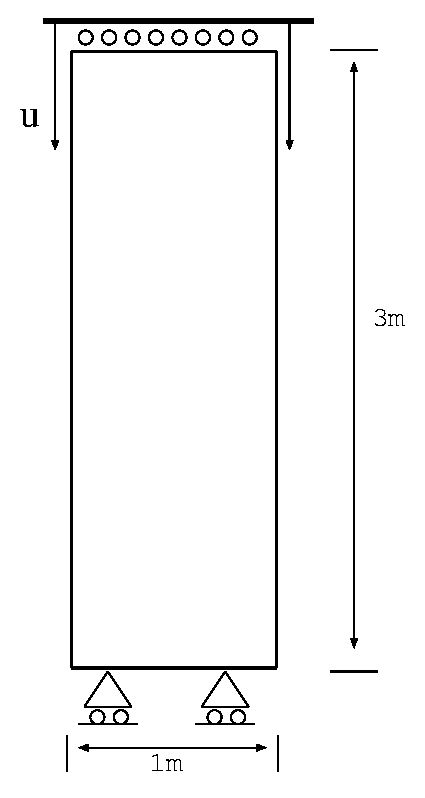
\includegraphics[scale=0.425]{PART_II/M/biaxial.eps}
\caption{Plane strain twodimensional localization test}
 \label{Mp_fig:biaxial}
\end{figure}

The bottom of the specimen is supported by horizontal roles, and its top surface is allowed to move only vertically with the axial displacement $u_z$. Both lateral surfaces are considered to be free of tractions.

The non-associative flow rule is adopted for the Drucker-Prager model with material parameters presented in Table~(\ref{Mp_ex1:tableDP}).

\subsubsection{Results}
\label{subsubsec:Mp2_res}

Fig.~\ref{Mp_fig:loc} shows the deformed model exhibiting localization. The stress response at the top surface to the prescribed displacements is discussed in Fig.~\ref{Mp_fig:vreact}. These results agree well with data presented in \cite{Bo00}.

\begin{table}[!htb]
\centering
\caption{Material parameters}
\label{Mp_ex1:tableDP}
\begin{tabular}{llll}
\toprule
Symbol & Parameter & Value & Unit \\
\midrule
$E$          & Young's modulus             & $20.0$     & MPa \\
$\nu$        & Poisson's ratio             & $0.4$      & --  \\
$\alpha$     & Factor in (\ref{Mp_eqn:dp}) & $0.233345$ & --  \\
$\beta$      & Factor in (\ref{Mp_eqn:dp}) & $0.141421$ & --  \\
$\sigma_0$   & Initial yield stress        & $29.69$    & kPa \\
$H$          & Hardening modulus           & $100$      & kPa \\
$H_{\delta}$ & Localized softening modulus & $-1000$    & kPa \\
\bottomrule
\end{tabular}
\end{table}
%
\begin{figure}[htb]
\begin{center}
\includegraphics[scale=0.3]{PART_II/M/m_sdc.eps}
\end{center}
\vspace*{-6.0ex}
\caption{Deformed contour with distribution of the axial displacements}
 \label{Mp_fig:loc}
\end{figure}
%
\begin{figure}[htb]
\begin{center}
\includegraphics[scale=0.3]{PART_II/M/m_sdc_s_u.eps}
\end{center}
\vspace*{-4.0ex}
\caption{Axial stress at the top as function of the axial displacement}
 \label{Mp_fig:vreact}
\end{figure}

\clearpage

